\documentclass[border=5pt]{standalone}
\usepackage{xcolor}
\usepackage{pgfplots}
\usepackage{tikz}

% Define bar chart colors
%
\definecolor{bblue}{HTML}{4F81BD}
\definecolor{rred}{HTML}{C0504D}
\definecolor{ggreen}{HTML}{9BBB59}
\definecolor{ppurple}{HTML}{9F4C7C}
\definecolor{orange}{HTML}{FF7E00}
\definecolor{yellow}{HTML}{FFFF66}

\pgfplotsset{every tick label/.append style={font=\large}}

\begin{document}
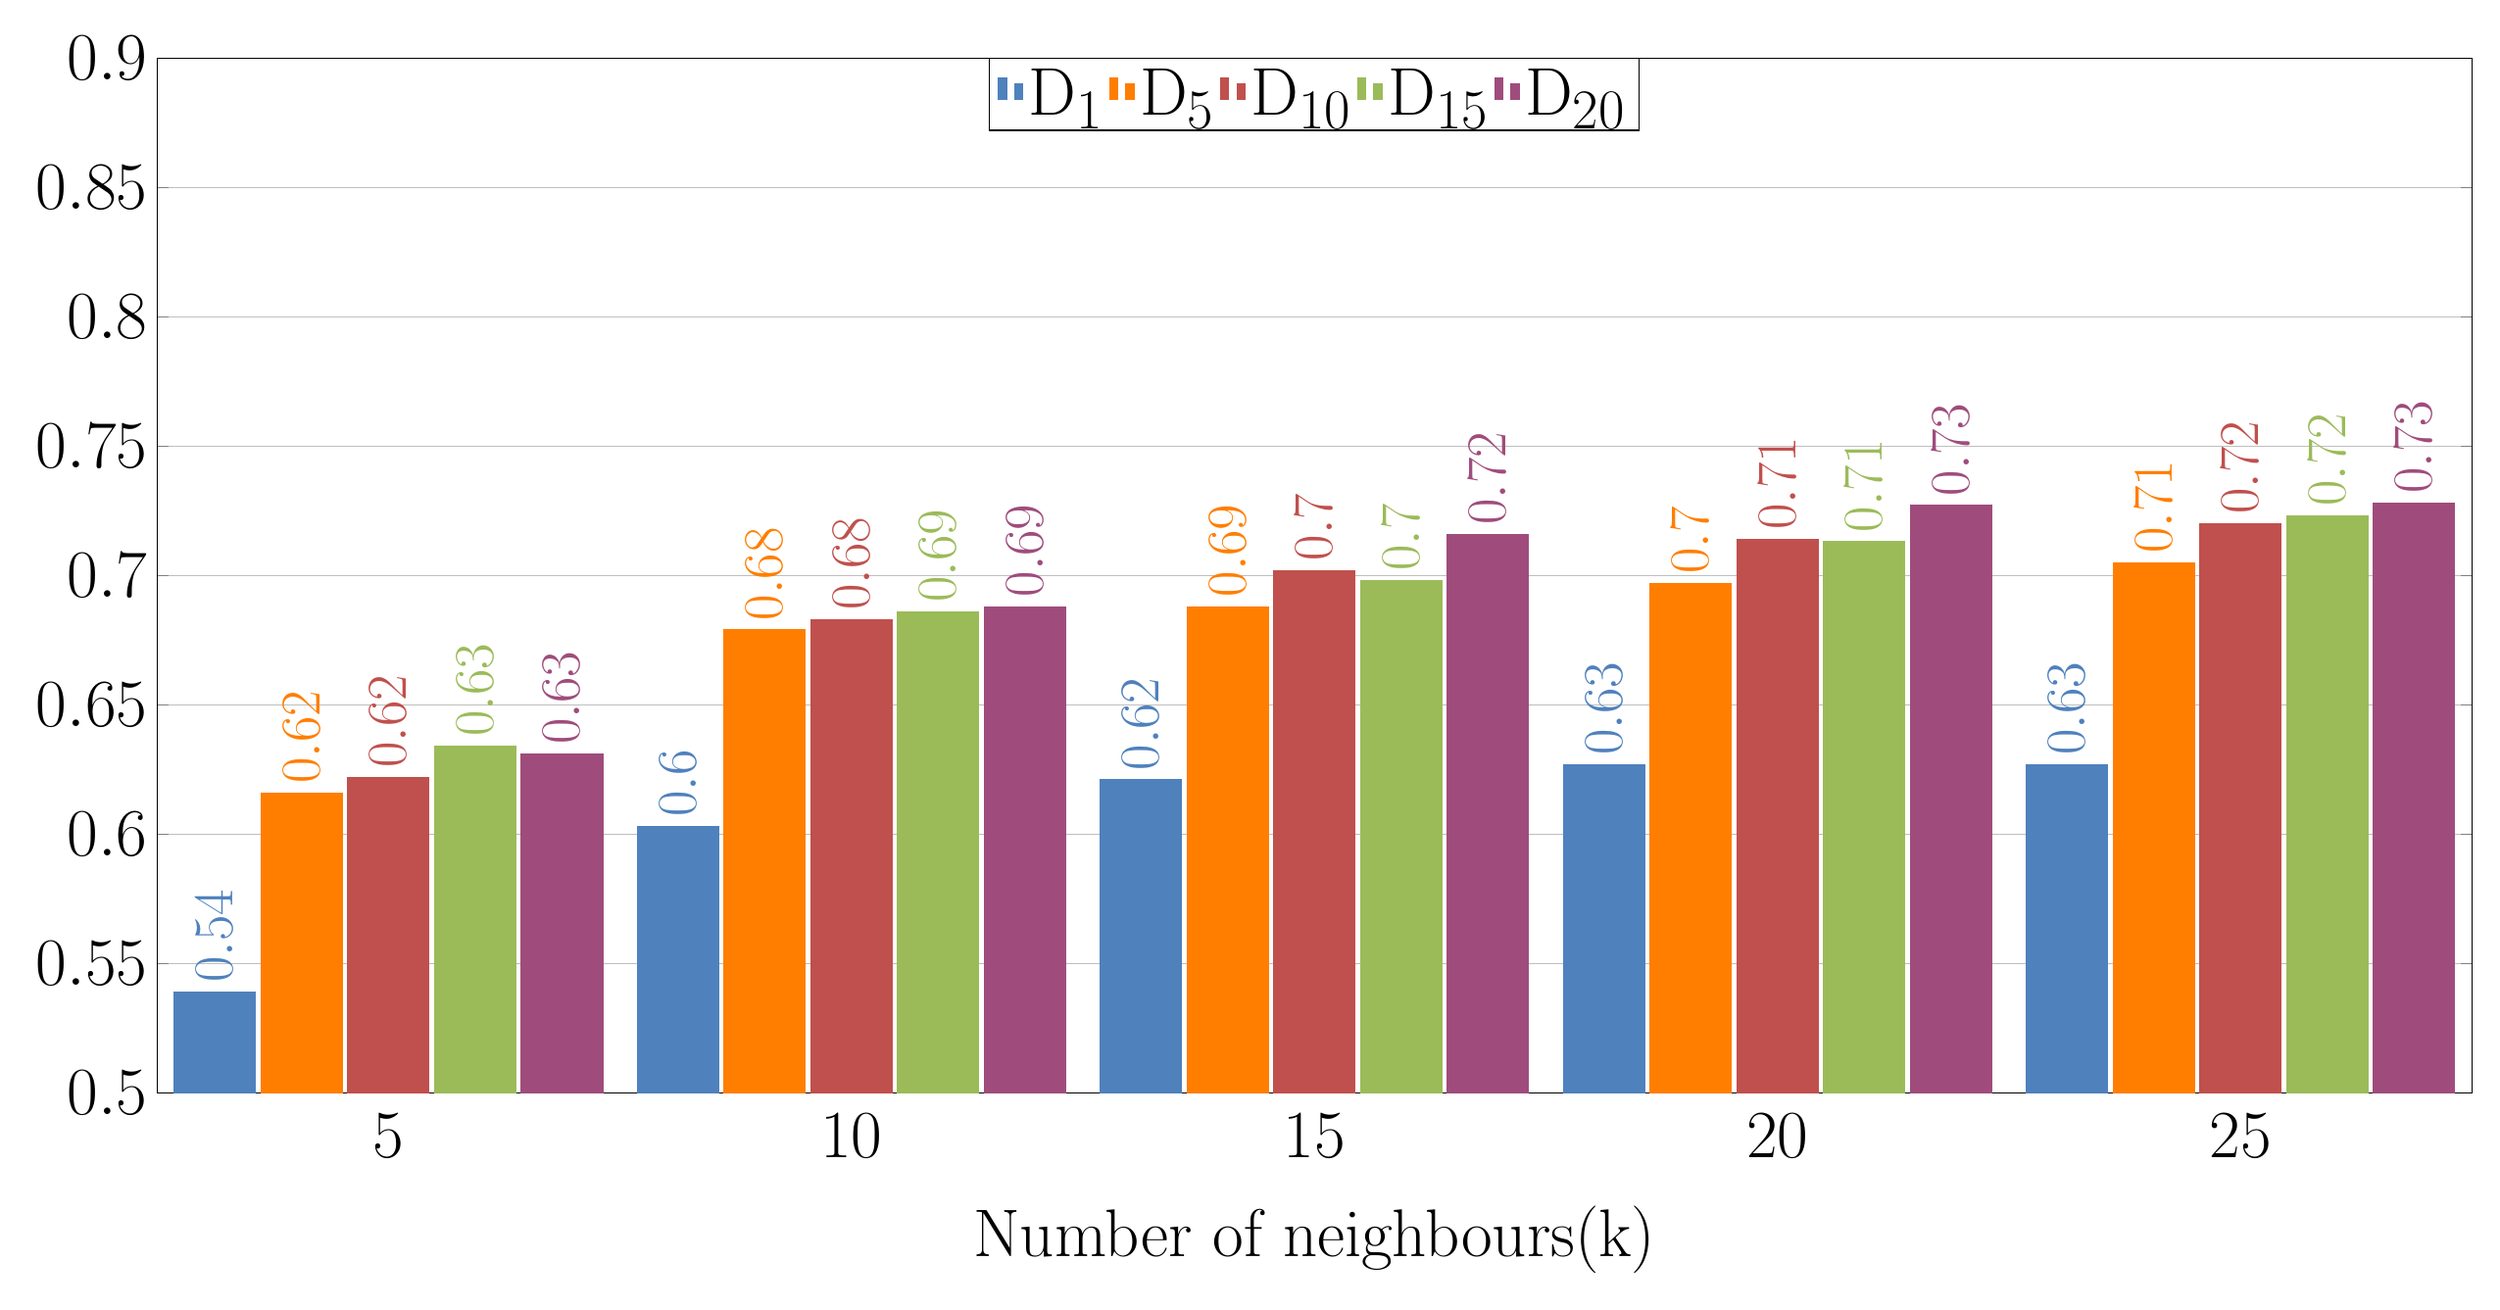
\begin{tikzpicture}
    \begin{axis}[
        width  = 6cm,%*\textwidth,
        height = 15	cm,
        major x tick style = transparent,
        ybar = 2pt,
        ymin = 0.5, ymax = 0.9,
        x=6cm,
        bar width=30pt,
        ymajorgrids = true,	
        xtick = data,
        scaled y ticks = false,
%		legend style={at={(0.5,-0.1)},
%		legend style={at={(0.5,1.1)}, anchor=north,legend columns=-1,font=\small},
      	legend style={at={(0.5,1)},	anchor=north,legend columns=-1,font=\Huge,
		anchor=north,legend columns=-1},
		enlarge x limits={abs=3cm},
		nodes near coords,
		nodes near coords style={font=\huge},
	    every node near coord/.append style={rotate=90, anchor=west},
	    xlabel={Number of neighbours(k)},
	    xlabel style={font=\Huge, at={(axis description cs:0.5,-0.1)},},
   	    every tick label/.append style={font=\Huge},
	    %ylabel = {Success rate@5 (\%)},	
        symbolic x coords={5,10,15,20,25},
    ]
        \addplot[style={bblue,fill=bblue,mark=none}]
            coordinates {(5, 0.539) (10, 0.603) (15,0.621)(20, 0.627)(25, 0.627)};
            
        \addplot[style={orange,fill=orange,mark=none}]
            coordinates {(5, 0.616) (10, 0.679) (15,0.688)(20, 0.697)(25, 0.705)};
                      
        \addplot[style={rred,fill=rred,mark=none}]
            coordinates {(5,0.622) (10,0.683) (15,0.702)(20,0.714)(25,0.720)};

        \addplot[style={ggreen,fill=ggreen,mark=none}]
            coordinates {(5,0.634) (10,0.686) (15, 0.698) (20,0.713) (25,0.723)};

        \addplot[style={ppurple,fill=ppurple,mark=none}]
            coordinates {(5,0.631) (10,0.688) (15,0.716) (20,0.727) (25,0.728)};

%      	\addplot[style={orange,fill=orange,mark=none}]
%            coordinates {(D$_1$,0.02) (10,0.902884311) (15,2.392886747)};
        \legend{D$_1$, D$_5$, D$_{10}$, D$_{15}$, D$_{20}$}
    \end{axis}
\end{tikzpicture}
\end{document}